\documentclass[paper=a4, fontsize=11pt]{scrartcl} % A4 paper and 11pt font size

\usepackage[T1]{fontenc} % Use 8-bit encoding that has 256 glyphs
\usepackage{fourier} % Use the Adobe Utopia font for the document - comment this line to return to the LaTeX default
\usepackage[english]{babel} % English language/hyphenation
\usepackage{amsmath,amsfonts,amsthm,amssymb} % Math packages

\usepackage{algorithm, algorithmic}
\renewcommand{\algorithmicrequire}{\textbf{Input:}} %Use Input in the format of Algorithm  
\renewcommand{\algorithmicensure}{\textbf{Output:}} %UseOutput in the format of Algorithm  

\usepackage{graphicx}

\usepackage{listings}
\lstset{language=Matlab}

\usepackage{lipsum} % Used for inserting dummy 'Lorem ipsum' text into the template

\usepackage{sectsty} % Allows customizing section commands
\allsectionsfont{\centering \normalfont\scshape} % Make all sections centered, the default font and small caps

\usepackage{fancyhdr} % Custom headers and footers
\pagestyle{fancyplain} % Makes all pages in the document conform to the custom headers and footers
\fancyhead{} % No page header - if you want one, create it in the same way as the footers below
\fancyfoot[L]{} % Empty left footer
\fancyfoot[C]{} % Empty center footer
\fancyfoot[R]{\thepage} % Page numbering for right footer
\renewcommand{\headrulewidth}{0pt} % Remove header underlines
\renewcommand{\footrulewidth}{0pt} % Remove footer underlines
\setlength{\headheight}{13.6pt} % Customize the height of the header

\numberwithin{equation}{section} % Number equations within sections (i.e. 1.1, 1.2, 2.1, 2.2 instead of 1, 2, 3, 4)
\numberwithin{figure}{section} % Number figures within sections (i.e. 1.1, 1.2, 2.1, 2.2 instead of 1, 2, 3, 4)
\numberwithin{table}{section} % Number tables within sections (i.e. 1.1, 1.2, 2.1, 2.2 instead of 1, 2, 3, 4)

\setlength\parindent{0pt} % Removes all indentation from paragraphs - comment this line for an assignment with lots of text

%----------------------------------------------------------------------------------------
%	TITLE SECTION
%----------------------------------------------------------------------------------------

\newcommand{\horrule}[1]{\rule{\linewidth}{#1}} % Create horizontal rule command with 1 argument of height

\title{	
\normalfont \normalsize 
\textsc{Shanghai Jiao Tong University, UM-SJTU JOINT INSTITUTE} \\ [25pt] % Your university, school and/or department name(s)
\horrule{0.5pt} \\[0.4cm] % Thin top horizontal rule
\huge Mechatronic Systems Design\\ HW1 \\ % The assignment title
\horrule{2pt} \\[0.5cm] % Thick bottom horizontal rule
}

\author{Yu Cang \quad 018370210001} % Your name

\date{\normalsize \today} % Today's date or a custom date

\begin{document}

\maketitle % Print the title

The autonomous drone is a new type of mechatronic system gaining popularity nowadays. 
\section{Hardware}
	Generally, it is based on the traditional multi-rotor configuration like Fig(\ref{fig:drone}), where 4 or 6 rotors are placed symmetrically around the central body. The central body contains power supply packages, controling unit and sensing facilities, with carbon fiber shell protecting them away from external dust, moist, or possible damage.
	
	\begin{figure}[!h]
		\centering
		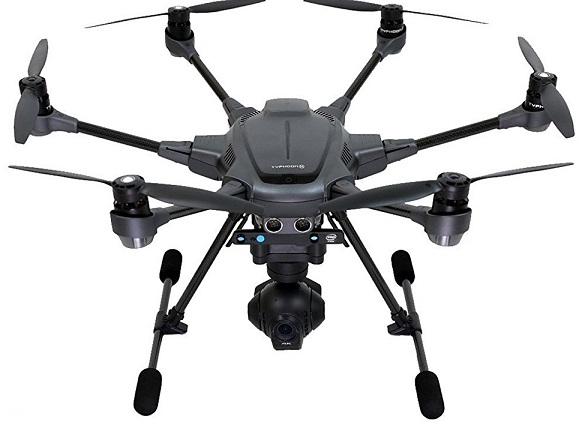
\includegraphics[width=5cm]{pic/drone.jpg}
		\caption{Autonomous drone}
		\label{fig:drone}
	\end{figure}

	Usually, a camera is mounted at the bottom for taking pictures or performing vision-based guiding.
	For professional use, both laser radar and milimeter-wave radar are equipped for advanced perception.
	
\section{Components}
	The most important 3 components are
	\begin{enumerate}
		\item \textbf{Sensing Unit}\\
			Usually, it is composed of accelerometer, gyroscope, barometer, geomagnetic sensor and GPS.These sensors are usually in chip format called MEMS, and can be mounted on the surface of PCB precisely, see Fig(\ref{fig:imu_pcb}).\\
			
			\begin{figure}[!h]
				\centering
				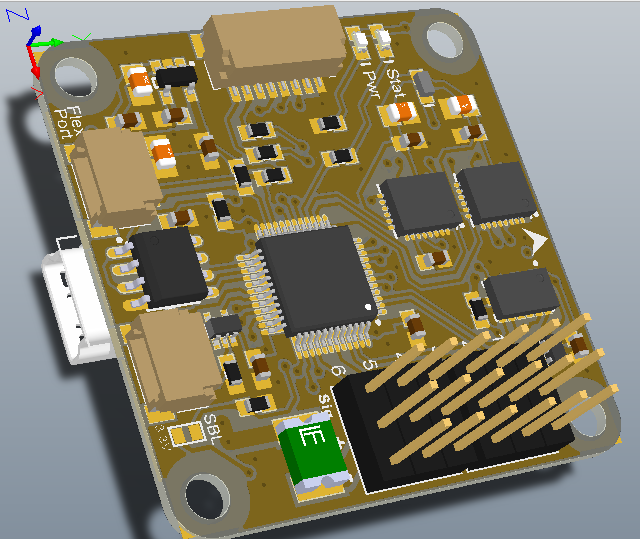
\includegraphics[width=5cm]{pic/imu.png}
				\caption{Sensing Unit PCB}
				\label{fig:imu_pcb}
			\end{figure}
			
			\begin{enumerate}
				\item \textit{Accelerometer}\\
					It provides the inertial force info, and 3-axis pose(Roll Yaw, Pitch) can be estimated from acceleration in each axis.
				\item \textit{Gyroscope}\\
					It provides the angular velocity info. It is based on the conservation of angular momentum.
				\item \textit{Barometer}\\
					It provide the pressure of atomosphere, and height can be estimated.
				\item \textit{Geomagnetic sensor}\\
					Guiding the \textbf{North} direction.
				\item \textit{GPS}\\
					Global position like longtitude and latitude are provided. Timing is also available.
			\end{enumerate}
		
			In general, sensing unit provides the state of drone. 
		
		\item \textbf{Perception Facility}\\
			To provide the infomation of environment, Radar, optical flow and ultrasonic sensor are integrated.
			
			\begin{enumerate}
				\item \textit{Laser Radar}\\
					Usually in shape like Fig(\ref{fig:lidar}), for sensing obstacles around. It can also be done using an RGB-D camera.
				\item \textit{Milimeter-wave Radar}\\
					Barometer may not accurate, Radar has better resolution on determining height.
				\item \textit{Optical Flow}\\
					Local positioning and velocity estimation.
				\item \textit{Ultrasonic sensor}\\
					Sensing in a specific direction, it has similar function as LiDAR but shorter range.
			\end{enumerate}
		
			\begin{figure}[!htbp]
				\centering
				\begin{minipage}[t]{0.48\textwidth}
					\centering
					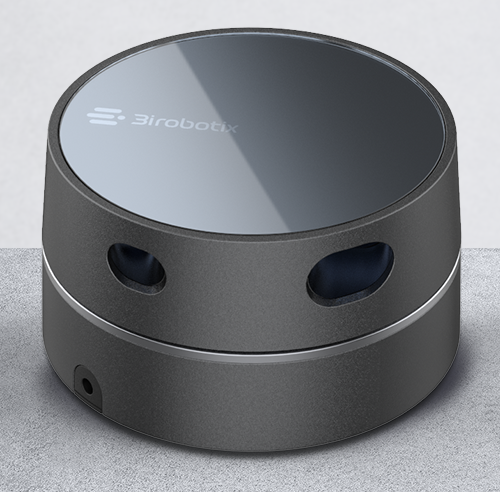
\includegraphics[width=5cm]{pic/lidar.png}
					\caption{LiDAR}
					\label{fig:lidar}
				\end{minipage}
				\begin{minipage}[t]{0.48\textwidth}
					\centering
					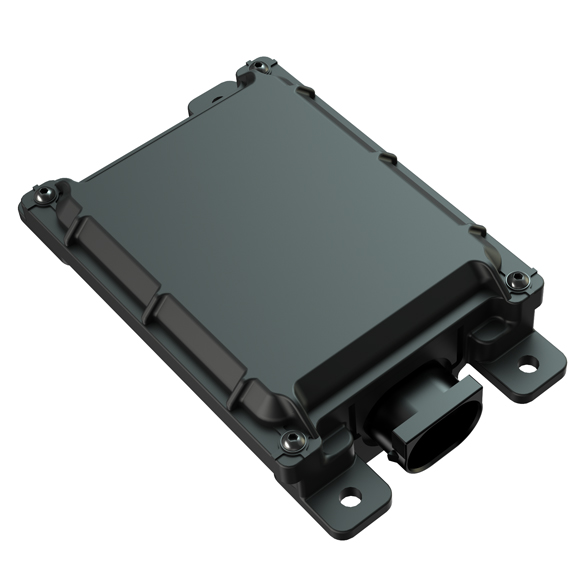
\includegraphics[width=5cm]{pic/radar.jpg}
					\caption{Milimeter-wave Radar}
					\label{fig:mm-wave}
				\end{minipage}
			\end{figure}
			
		\item \textbf{Control Unit}\\
			It do realtime response under both internal and external constraints. Signals in PWM form are generated to the electrical speed regulator to drive the motors. Usually, serial PID algorithm is used.
			
	\end{enumerate}

\section{Specifications}
	Usually, this kind of automous drones can be used for agricultural, topographic or transportation purpose. Typically, the diameter ranges from 0.5 to 2m, and weighs 2 to 20kg.\\
	Due to the energy density limit of lithium battery, endurance is usually about 20 minutes.\\
	For safety issues, flight speed is usually lower than 5m/s, and flight height is restricted to 10m.

\section{Challenges in design and control}
	\begin{enumerate}
		\item 
			Data fusion.
		\item 
			Proper placement to minimize vibration.
		\item 
			PID param tuning.
		\item 
			Obstacle detection.
		\item 
			Reliable wireless communication.
	\end{enumerate}

\section{Future trends of developments}
	\begin{enumerate}
		\item 
			Communication for long range and high fidelity.
		\item 
			Advanced and robust control algorithm.
		\item 
			Optimized aerodynamic shape design(For agricultural spray).
		\item 
			Higher energy density batteries or use gasoline.
		\item 
			More mature environment perception.
	\end{enumerate}

\end{document}
